% =============================================================================
% COPYRIGHT AND DISCLAIMER
% =============================================================================
% This file is provided as a convenience template for competition participants.
% By using it, you accept full responsibility for compliance with all applicable
% copyright, licensing, and usage rules of the Association for Computing
% Machinery (ACM) and of any LaTeX packages you load (including, without
% limitation, the "acmart" document class and related ACM materials).
%
% Consult ACM's official publication, template, and copyright policies before
% using this setup for any purpose other than this competition. Do not assume
% that this template may be reused, redistributed, or submitted elsewhere
% without independently verifying ACM's current rules.
%
% Use of the "acmart" class, the "sigconf" option, or ACM-style formatting in
% this template does NOT mean that this report, this competition, its organizers,
% or any resulting PDF is sponsored, endorsed, affiliated with, or published by
% ACM. ACM trademarks and branding remain the property of ACM.
%
% Template packages live in preamble.tex.
% Citations live in main.bib. Edit this file with your paper content.
% =============================================================================

\documentclass[sigconf]{acmart}
% =============================================================================
% Template setup — participants normally do not edit this file.
% Author content belongs in main.tex; citations belong in main.bib.
% \documentclass lives in main.tex so Overleaf does not treat this file as root.
% =============================================================================

% --- Competition / non-ACM-submission friendly rights metadata -------------
\setcopyright{none}
\settopmatter{printacmref=false}
\acmConference[Kaggle Competition]{Filament Segmentation Challenge}{2026}{\href{https://www.kaggle.com/competitions/filament-segmentation-2026}{kaggle.com/competitions/filament-segmentation-2026}}
\acmBooktitle{Competition Report}
\acmDOI{}
\acmISBN{}

% --- Author guidance text --------------------------------------------------
% \guide{...} is gray italic while \guideStyletrue; omitted from the PDF if false.
% Flip the switch in main.tex after % =============================================================================
% Template setup — participants normally do not edit this file.
% Author content belongs in main.tex; citations belong in main.bib.
% \documentclass lives in main.tex so Overleaf does not treat this file as root.
% =============================================================================

% --- Competition / non-ACM-submission friendly rights metadata -------------
\setcopyright{none}
\settopmatter{printacmref=false}
\acmConference[Kaggle Competition]{Filament Segmentation Challenge}{2026}{\href{https://www.kaggle.com/competitions/filament-segmentation-2026}{kaggle.com/competitions/filament-segmentation-2026}}
\acmBooktitle{Competition Report}
\acmDOI{}
\acmISBN{}

% --- Author guidance text --------------------------------------------------
% \guide{...} is gray italic while \guideStyletrue; omitted from the PDF if false.
% Flip the switch in main.tex after % =============================================================================
% Template setup — participants normally do not edit this file.
% Author content belongs in main.tex; citations belong in main.bib.
% \documentclass lives in main.tex so Overleaf does not treat this file as root.
% =============================================================================

% --- Competition / non-ACM-submission friendly rights metadata -------------
\setcopyright{none}
\settopmatter{printacmref=false}
\acmConference[Kaggle Competition]{Filament Segmentation Challenge}{2026}{\href{https://www.kaggle.com/competitions/filament-segmentation-2026}{kaggle.com/competitions/filament-segmentation-2026}}
\acmBooktitle{Competition Report}
\acmDOI{}
\acmISBN{}

% --- Author guidance text --------------------------------------------------
% \guide{...} is gray italic while \guideStyletrue; omitted from the PDF if false.
% Flip the switch in main.tex after \input{preamble}.
%
% Do not use \guide{...} for \email{...}.
\usepackage{xcolor}
\newif\ifguideStyle
\guideStyletrue
\newcommand{\guide}[1]{%
  \ifguideStyle
    {\color{gray!65}\itshape #1}%
  \fi
}

% --- Math ------------------------------------------------------------------
% Do NOT load amssymb (or amsfonts): acmart already loads newtxmath, which
% defines the same symbols (e.g. \Bbbk) and causes a conflict on Overleaf.
% amsmath is already provided by acmart; mathtools extends it.
\usepackage{mathtools}

% --- Figures ---------------------------------------------------------------
% graphicx is already loaded by acmart
\usepackage{subcaption}

% --- Tables ----------------------------------------------------------------
% booktabs is already loaded by acmart
\usepackage{tabularx}
\usepackage{multirow}

% --- Bibliography style is set in main.tex (ACM-Reference-Format) ----------

% Let TeX stretch spacing slightly instead of pushing a line into the margin
% (only applies to paragraphs that cannot otherwise be set without overflow).
\setlength{\emergencystretch}{1.5em}
.
%
% Do not use \guide{...} for \email{...}.
\usepackage{xcolor}
\newif\ifguideStyle
\guideStyletrue
\newcommand{\guide}[1]{%
  \ifguideStyle
    {\color{gray!65}\itshape #1}%
  \fi
}

% --- Math ------------------------------------------------------------------
% Do NOT load amssymb (or amsfonts): acmart already loads newtxmath, which
% defines the same symbols (e.g. \Bbbk) and causes a conflict on Overleaf.
% amsmath is already provided by acmart; mathtools extends it.
\usepackage{mathtools}

% --- Figures ---------------------------------------------------------------
% graphicx is already loaded by acmart
\usepackage{subcaption}

% --- Tables ----------------------------------------------------------------
% booktabs is already loaded by acmart
\usepackage{tabularx}
\usepackage{multirow}

% --- Bibliography style is set in main.tex (ACM-Reference-Format) ----------

% Let TeX stretch spacing slightly instead of pushing a line into the margin
% (only applies to paragraphs that cannot otherwise be set without overflow).
\setlength{\emergencystretch}{1.5em}
.
%
% Do not use \guide{...} for \email{...}.
\usepackage{xcolor}
\newif\ifguideStyle
\guideStyletrue
\newcommand{\guide}[1]{%
  \ifguideStyle
    {\color{gray!65}\itshape #1}%
  \fi
}

% --- Math ------------------------------------------------------------------
% Do NOT load amssymb (or amsfonts): acmart already loads newtxmath, which
% defines the same symbols (e.g. \Bbbk) and causes a conflict on Overleaf.
% amsmath is already provided by acmart; mathtools extends it.
\usepackage{mathtools}

% --- Figures ---------------------------------------------------------------
% graphicx is already loaded by acmart
\usepackage{subcaption}

% --- Tables ----------------------------------------------------------------
% booktabs is already loaded by acmart
\usepackage{tabularx}
\usepackage{multirow}

% --- Bibliography style is set in main.tex (ACM-Reference-Format) ----------

% Let TeX stretch spacing slightly instead of pushing a line into the margin
% (only applies to paragraphs that cannot otherwise be set without overflow).
\setlength{\emergencystretch}{1.5em}


% Guide styling: \guideStyletrue = show gray italic hints; \guideStylefalse = omit them
% \guideStyletrue
\guideStylefalse

% Numbers that come from scripts (docs/logs/final/): keep them in one place.
\newcommand{\pqoof}{0.4372}        % final 1, 707 OOF images, post-processing and filter tuned on OOF
\newcommand{\pqcross}{0.4339}      % final 1 maps, post-processing cross-tuned across folds
\newcommand{\pqci}{[0.427, 0.447]} % bootstrap 95% CI of \pqoof over images (report_stats.json)
\newcommand{\dicemean}{0.663}      % rubric_final1.json
\newcommand{\tpiou}{0.680}
\newcommand{\onen}{3.1}
\newcommand{\none}{3.9}

\begin{document}

\title{Three U-Net Families, Hysteresis and Oriented Grouping for Filament Instance Segmentation}
\subtitle{A Solution to the Solar Filament Segmentation Challenge 2026} % DO NOT CHANGE

\author{Cuong Nguyen}
\affiliation{%
  \country{Vietnam}
}
\email{nguyenchicuong.ai@gmail.com}

\begin{abstract}
    This report describes our solution to the Solar Filament Segmentation Challenge~2026, a Kaggle competition on automatic segmentation of solar filaments in GONG H-$\alpha$ observations. Our pipeline averages the probability maps of 15 U-Nets (three encoder/scale families, five folds each) trained on soft multi-annotator targets, then turns the map into instances with hysteresis thresholding, orientation-aware fragment grouping and a gradient-boosted false-positive filter. All choices were made on out-of-fold Panoptic Quality (PQ) over the 707 training images with paired bootstrap tests, never on the public leaderboard. The final pipeline reaches PQ~\pqoof{} out of fold (\pqcross{} with cross-tuned post-processing), above the 0.340 PQ that one human annotator scores against another, and 0.38 on the public leaderboard. Inference needs only the test images and runs end to end in a public notebook.
\end{abstract}

\maketitle

% ==================================== %
%              INTRODUCTION            %
% ==================================== %
\section{Introduction}
    This report goes over the details of our submitted solution to the Solar Filament Segmentation Challenge~2026 \cite{filament-segmentation-2026}. The challenge, launched on July~10,~2026, is organized by the Earth-Space AI Research (ESAIR) Lab\footnote{\href{https://www.esairlab.com/home}{www.esairlab.com/}}. This challenge utilizes the MAGFiLO dataset for evaluation of the segmentation algorithms \cite{ahmadzadeh2024dataset}. The metric is Panoptic Quality \cite{kirillov2019panoptic} with matches at IoU~$>0.5$, computed separately against every annotator of an image and pooled over all annotator entries. Two properties of the data shaped our design: (i) annotators disagree strongly (one annotator scored against another reaches only PQ~0.340, SQ~0.634 on the multi-annotator training images), so the target is an ``average annotator'' rather than a crisp truth; and (ii) a filament split into two pieces costs one TP and adds two FPs, so instance separation matters as much as mask quality. Code, weights and the end-to-end notebook are in our repository\footnote{\url{https://github.com/nguyenchicuongvn/filament-segmentation-2026} (MIT license).}.

% ==================================== %
%              METHODOLOGY             %
% ==================================== %
\section{Methodology}\label{sec:methodology}

\begin{figure*}[t]
  \centering
  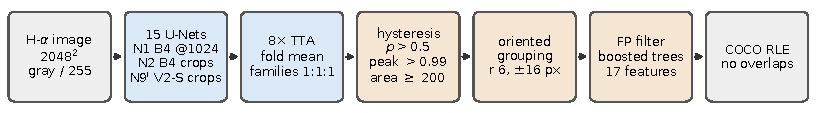
\includegraphics[width=\textwidth]{figures/pipeline.pdf}
  \caption{End-to-end pipeline. Only the test H-$\alpha$ image is used at inference. Blue: networks and map ensembling; orange: post-processing tuned on out-of-fold maps.}
  \label{fig:pipeline}
\end{figure*}

\subsection{Data, splits and selection protocol}
The training set has 707 images ($2048\times2048$, three identical channels read as one gray channel), 1{,}154 annotator entries and 8{,}199 filaments; 411 images have one annotator, 145 two and 151 three. We use only the masks (no bounding boxes, spines or chirality labels). We split the images into five folds by \emph{image} (seed~42), so all annotators of an image fall in the same fold; an earlier split by entry had leaked images between train and validation. Every model is trained five times, once per held-out fold, and the held-out maps form an out-of-fold (OOF) prediction for all 707 images and 1{,}154 entries. All decisions use OOF PQ: a change is accepted only if the paired bootstrap over images (2{,}000 resamples) gives a 95\% CI above zero, with the acceptance rule written down before the numbers were seen. Post-processing parameters are \emph{cross-tuned} when comparing pipelines (chosen on four folds, scored on the fifth) so that pipelines with more knobs are not favoured. The public leaderboard (about 90 images, two decimals) was used only to confirm reproducibility, never to choose.

\subsection{Targets and training}
For each image the target is \emph{soft}: the fraction of the image's annotators whose filaments cover the pixel (0, 1/3, 1/2, 2/3, 1). Each epoch draws images with probability proportional to their number of annotators, which matches how the metric weights entries. Inputs are scaled to $[0,1]$; we apply no physical preprocessing, because the GONG images are already limb-corrected and normalised (median disk intensity 130--133 at all six stations, same in train and test) and model errors did not depend on disk position. Augmentation is a random $90^\circ$ rotation and a horizontal flip. Crops are centred on a random filament pixel with probability 0.7, otherwise uniform.

All networks are U-Nets \cite{ronneberger2015unet} from \texttt{segmentation-models-pytorch} 0.5.0 \cite{iakubovskii2019smp} with ImageNet-pretrained encoders (EfficientNet-B4 \cite{tan2019efficientnet}; EfficientNetV2-S \cite{tan2021efficientnetv2} from \texttt{timm} \cite{wightman2019timm}, ImageNet-21k weights), one output channel and a sigmoid. The loss is binary cross-entropy plus soft Dice on the soft target. We train with AdamW (weight decay $10^{-4}$), a one-cycle schedule with 5\% warm-up, mixed precision, and keep the last checkpoint. Table~\ref{tab:families} lists the three families; N2 and N9$'$ see native-resolution crops and are applied to the full $2048\times2048$ image at test time (the networks are fully convolutional).

\begin{table}[t]
  \caption{The three U-Net families (five folds each). Time is per fold.}
  \label{tab:families}
  \small
  \begin{tabular}{@{}llllll@{}}
    \toprule
    & Encoder & Input & Batch, LR & Steps & GPU time \\
    \midrule
    N1 & EffNet-B4 & full image @1024 & 4, $10^{-3}$ & 6.9k & 2.0\,h T4 \\
    N2 & EffNet-B4 & 1024 crops @2048 & 4, $10^{-3}$ & 6.9k & 1.8\,h T4 \\
    N9$'$ & EffNetV2-S & 512 crops @2048 & 16, $3\cdot10^{-4}$ & 10.5k & 1.3\,h L4 \\
    \bottomrule
  \end{tabular}
\end{table}

\subsection{Inference and map ensembling}
Each checkpoint predicts with 8-fold test-time augmentation (four rotations $\times$ flip, averaged). The five fold models of a family are averaged, N1 maps are upsampled bilinearly from 1024 to 2048, and the three family maps are averaged 1:1:1 (maps are stored as \texttt{uint8}). Weighting N9$'$ twice ($-0.0007$ [$-0.0025$, $+0.0010$]) or N1 twice did not help.

\subsection{Post-processing}
\emph{Hysteresis.} Pixels with $p>0.5$ form 8-connected components; a component is kept if its area is at least 200~px and its peak probability exceeds 0.99, so faint regions survive only when attached to a confident core (in the spirit of Canny's hysteresis \cite{canny1986}). \emph{Oriented grouping.} Filaments are often thin and broken into collinear pieces. Each kept component is dilated by a disk of radius 6 united with a line segment of $\pm16$~px along its major axis (from second moments); components whose dilations touch become one instance, and the instance keeps only the original pixels, so masks never overlap. \emph{False-positive filter.} For every instance we compute 17 features (log area, mean/max/25th-percentile probability, fraction of confident pixels, extent, elongation, major-axis length, contrast and mean gray level, radius on the disk, number and area rank of instances in the image, $|x|$, $y$ and $|$longitude$|$ on the disk, since annotators skip filaments beyond about $70^\circ$ from the central meridian). A gradient-boosted classifier (scikit-learn \texttt{HistGradientBoosting}, \cite{ke2017lightgbm}) predicts whether the instance matches some annotator at IoU~$>0.5$; its scores are cross-validated by image, and instances scoring below 0.375 (the value that maximises OOF PQ) are dropped. Instances are then upsampled to 2048 and written as COCO RLE. Figure~\ref{fig:examples} shows OOF examples.

\begin{figure*}[t]
  \centering
  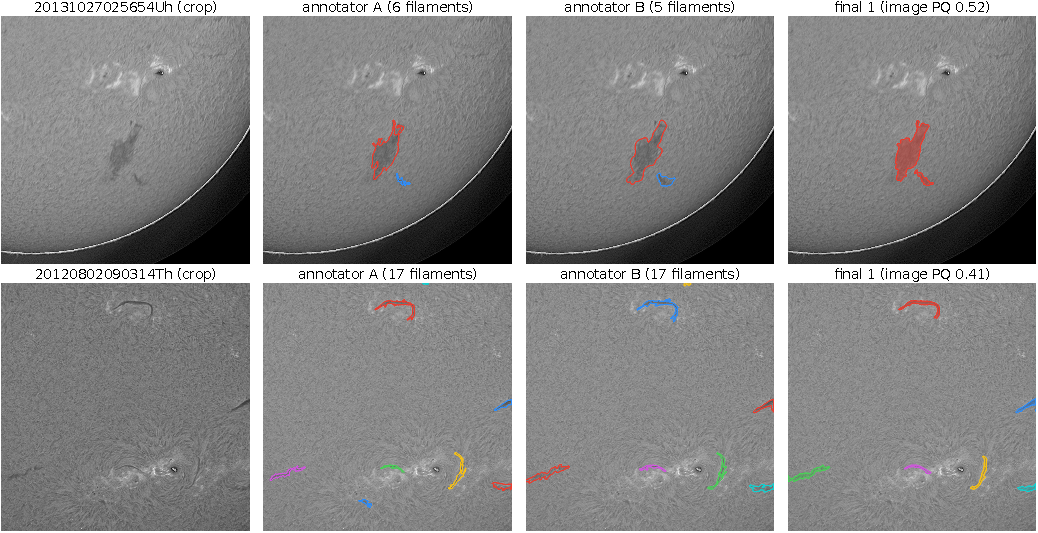
\includegraphics[width=\textwidth]{figures/examples.pdf}
  \caption{Out-of-fold examples ($900\times900$ crops of two training images with two annotators each). Outlines: annotators' filaments; filled: final instances, one colour per instance. Note how much the annotators differ.}
  \label{fig:examples}
\end{figure*}

% ==================================== %
%              EVALUATION              %
% ==================================== %
\section{Evaluation}\label{sec:evaluation}

\subsection{Strategy}
We report OOF PQ on all 707 training images (1{,}154 entries), with the metric of the host's self-evaluation notebook re-implemented and unit-tested, and the public leaderboard score of the same pipeline trained on all folds. Uncertainties are bootstrap 95\% intervals over images. The OOF PQ of the final pipeline is \pqoof{} \pqci{} (4{,}839 TP, 2{,}006 FP, 3{,}360 FN pooled over entries); the filter decisions in this number are out of fold (the filter is refitted with each image's fold held out), only its threshold was chosen on these scores. The five per-fold values range from 0.425 to 0.454, consistent with the bootstrap SD of 0.005 for 707 images and about 0.011 for one fold.

\subsection{Results and ablations}
Table~\ref{tab:results} builds the final pipeline one step at a time. Each row's $\Delta$ is the paired difference to the row it modifies, with cross-tuned post-processing. The largest single gains came from the soft multi-annotator target with five folds (N1), from averaging families that see the image at different scales (N1+N2: FP $-222$ at almost unchanged TP), and from hysteresis (removing it costs $-0.024$ OOF and 0.02 on the leaderboard). Grouping broken pieces is the other post-processing step the leaderboard can see (without it: $-0.006$ OOF, $-0.01$ LB); a plain disk of radius 12 instead of the oriented kernel is slightly worse ($-0.001$ on final~1, $-0.002$ [$-0.004$, $-0.001$] on N1+N2). Dropping N2 from the final pool is neutral ($+0.002$, CI includes 0), so N2's contribution is absorbed by N9$'$, which also sees native-resolution crops; we kept the pre-registered pool. On the test set, one fold model per family (3 models) already scores 0.38 like the 15-model pool, while a single N9$'$ model scores 0.37 (fold-0 PQ 0.427 against 0.442 for the three). The leaderboard has a resolution of about 0.01 on 90 images (bootstrap SD 0.014), so differences below 0.01 are not visible there; the ordering of OOF and leaderboard agrees wherever the leaderboard can resolve it.

\begin{table}[t]
  \caption{Building the final pipeline: OOF PQ on 707 images (cross-tuned post-processing unless noted), paired bootstrap 95\% CI, and public leaderboard.}
  \label{tab:results}
  \small
  \begin{tabular}{@{}lllc@{}}
    \toprule
    Pipeline & OOF PQ & $\Delta$ [95\% CI] & LB \\
    \midrule
    N1 single family & 0.4179 & -- & 0.37 \\
    N2 single family & 0.4129 & $-0.005$ [$-0.010$, $-0.0003$] & 0.37 \\
    N1 + N2 & 0.4284 & $+0.011$ [$+0.007$, $+0.014$] & 0.37 \\
    N1 + N2 + N9$'$ & 0.4339 & $+0.006$ [$+0.003$, $+0.008$] & 0.38 \\
    \quad tuned on all OOF & 0.4354 & in-sample & 0.38 \\
    \quad + FP filter (final 1) & \textbf{0.4372} & $+0.002$, CV filter & \textbf{0.38} \\
    \midrule
    \multicolumn{4}{@{}l}{\emph{Ablations and single families}} \\
    final 1 without hysteresis$^*$ & 0.4119 & $-0.024$ vs.\ 0.4354 & 0.36 \\
    N1+N2 without hysteresis$^\dagger$ & 0.4065 & $-0.025$ [$-0.029$, $-0.020$] & 0.36 \\
    disk grouping (r 12) instead of oriented$^*$ & 0.4344 & $-0.001$ [$-0.003$, $+0.001$] & 0.38 \\
    no grouping$^*$ & 0.4293 & $-0.006$ [$-0.011$, $-0.002$] & 0.37 \\
    plain threshold 0.5 (no hysteresis, grouping)$^*$ & 0.3985 & $-0.037$ [$-0.043$, $-0.031$] & 0.35 \\
    final 1 without N2$^*$ & 0.4371 & $+0.002$ [$-0.001$, $+0.004$] & 0.38 \\
    final 1 without N1$^*$ & 0.4262 & $-0.009$ [$-0.013$, $-0.006$] & 0.38 \\
    N9$'$ single family & 0.4192$^*$ & -- & 0.38 \\
    ResNet34, N9$'$ recipe & 0.3955$^*$ & -- & 0.36 \\
    \bottomrule
  \end{tabular}

  \smallskip
  \footnotesize $^\dagger$on N1+N2, cross-tuned, no filter. $^*$post-processing tuned on all OOF, no filter.
\end{table}

\subsection{Host rubric metrics and cost}
Figure~\ref{fig:rubric} gives the rubric's distributions for the final pipeline on the OOF entries: mean Dice \dicemean{} (\texttt{torchmetrics} \texttt{DiceScore}, one value per annotator entry), mean IoU of matched pairs \tpiou, and \onen\% of ground-truth filaments touched by two or more predictions (1:n) against \none\% of predictions touching two or more filaments (n:1). End-to-end inference of 180 test images (15 models $\times$ 8 TTA at 2048) takes 90 minutes on a Kaggle machine with two T4 GPUs, about 30\,s per image; post-processing and the filter add under 1\,s per image on CPU. Training all 15 models takes about 25 GPU-hours.

\begin{figure}[t]
  \centering
  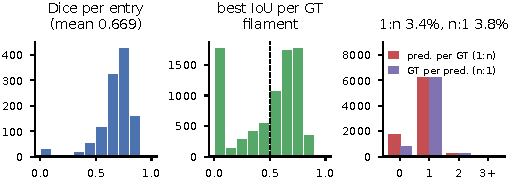
\includegraphics[width=\columnwidth]{figures/rubric.pdf}
  \caption{Rubric distributions of final 1 on 1{,}154 OOF annotator entries: Dice per entry, best IoU of each ground-truth filament (dashed: match threshold), and one-to-many / many-to-one counts (any shared pixel).}
  \label{fig:rubric}
\end{figure}

\subsection{Strengths, weaknesses and what did not work}
\emph{Strengths.} The pipeline is simple (three U-Net families and four classical post-processing steps), every component was accepted by a pre-registered OOF test, and it is fully reproducible: a Kaggle kernel rebuilt both final submissions from the repository and the test images alone; the N1+N2 submission matched byte for byte, and final~1 scored the same leaderboard value.

\emph{Weaknesses.} Decomposing $1-\mathrm{PQ}$ on OOF gives 36\% boundary error, 38\% false negatives and 26\% false positives. Most remaining error is annotator disagreement: 34\% of our false positives coincide with a filament drawn by another annotator of the same image, 38\% of false negatives are filaments that only one annotator drew, and filaments below 1{,}000~px are missed 54\% of the time (humans miss small filaments of each other at a similar rate). Turning near-misses (IoU 0.3--0.5) into matches would be worth up to $+0.055$, fixing merges $+0.028$ and splits $+0.015$; dropping every FP that touches no annotator only $+0.010$.

\emph{Negative results} (OOF, cross-tuned): a second seed of N9$'$ as a fourth family ($-0.003$ [$-0.005$, $-0.001$]), a ResNet34 family with the N9$'$ recipe ($-0.0004$ [$-0.002$, $+0.001$]), a BCE-only family ($+0.002$, CI includes 0), blob-Dice and false-component losses ($-0.05$ on two folds), ConvNeXt-T ($-0.020$), watershed splitting ($0.000$), a Mask R-CNN at 512 px ($-0.158$ alone, $-0.006$ fused), multi-scale TTA ($-0.003$) and size-dependent mask growth (no gain on top of hysteresis).

\emph{Improvements.} Since the boundary and grouping errors are bounded by annotator variance, the most promising direction is to model each annotator group explicitly (e.g. conditional heads) and to learn grouping from instance embeddings instead of a fixed oriented dilation.

% ==================================== %
%            ACKNOWLEDGMENT            %
% ==================================== %
\section{Acknowledgment}\label{sec:acknowledgment}
    % Do not change
    The organization of the Filament Segmentation Challenge 2026 is partially supported by the U.S. National Science Foundation (NSF) under Grant No. 2209912 and 2433781, directorate for Computer and Information Science and Engineering (CSE), and Office of Advanced Cyberinfrastructure (OAC), and Grant No. 2511630, AST Division Of Astronomical Sciences and MPS Directorate for Mathematical and Physical Sciences.

    The Filament Segmentation Challenge 2026 is sponsored by the U.S. National Science Foundation (NSF) National Solar Observatory (NSO).

    This work utilizes GONG data obtained by the NSO Integrated Synoptic Program, managed by the National Solar Observatory, which is operated by the Association of Universities for Research in Astronomy (AURA), Inc. under a cooperative agreement with the National Science Foundation and with contribution from the National Oceanic and Atmospheric Administration. The GONG network of instruments is hosted by the Big Bear Solar Observatory, High Altitude Observatory, Learmonth Solar Observatory, Udaipur Solar Observatory, Instituto de Astrofísica de Canarias, and Cerro Tololo Interamerican Observatory.

\bibliographystyle{ACM-Reference-Format}
\bibliography{main}

\end{document}
